

%  article.tex (Version 3.3, released 19 January 2008)
%  Article to demonstrate format for SPIE Proceedings
%  Special instructions are included in this file after the
%  symbol %>>>>
%  Numerous commands are commented out, but included to show how
%  to effect various options, e.g., to print page numbers, etc.
%  This LaTeX source file is composed for LaTeX2e.

%  The following commands have been added in the SPIE class 
%  file (spie.cls) and will not be understood in other classes:
%  \supit{}, \authorinfo{}, \skiplinehalf, \keywords{}
%  The bibliography style file is called spiebib.bst, 
%  which replaces the standard style unstr.bst.  

\documentclass[a4paper]{spie}  %>>> use for US letter paper
%%\documentclass[a4paper]{spie}  %>>> use this instead for A4 paper
%%\documentclass[nocompress]{spie}  %>>> to avoid compression of citations
%% \addtolength{\voffset}{9mm}   %>>> moves text field down
%% \renewcommand{\baselinestretch}{1.65}   %>>> 1.65 for double spacing, 1.25 for 1.5 spacing 
%  The following command loads a graphics package to include images 
%  in the document. It may be necessary to specify a DVI driver option,
%\textit{}%  e.g., [dvips], but that may be inappropriate for some LaTeX 

%  installations. 
\usepackage{amsmath}
\usepackage[]{graphicx}
\usepackage{hyperref}
\usepackage{listings}
\hypersetup{
    colorlinks,
    linkcolor={black!50!black},
    citecolor={blue!50!black},
    urlcolor={blue!80!black}
}
\usepackage{pdfpages}
\usepackage{parcolumns}

\usepackage[utf8]{inputenc} 
\usepackage[ngerman]{babel}
\usepackage[autostyle=true,german=quotes]{csquotes}

\usepackage{color}
\definecolor{lightgray}{rgb}{.9,.9,.9}
\definecolor{darkgray}{rgb}{.4,.4,.4}
\definecolor{purple}{rgb}{0.65, 0.12, 0.82}


\usepackage{array}
\newcolumntype{L}[1]{>{\raggedright\let\newline\\\arraybackslash\hspace{0pt}}m{#1}}
\newcolumntype{C}[1]{>{\centering\let\newline\\\arraybackslash\hspace{0pt}}m{#1}}
\newcolumntype{R}[1]{>{\raggedleft\let\newline\\\arraybackslash\hspace{0pt}}m{#1}}

\usepackage[export]{adjustbox}
\usepackage{xcolor,colortbl}
\usepackage{color}
\usepackage{float}

\definecolor{lightgray}{rgb}{.9,.9,.9}
\definecolor{darkgray}{rgb}{.4,.4,.4}
\definecolor{purple}{rgb}{0.65, 0.12, 0.82}
% Farben definieren
\definecolor{codeGray}{RGB}{240,240,240}
\definecolor{codeBlack}{RGB}{0,0,0}
\definecolor{codeRed}{RGB}{221,0,0}
\definecolor{codeBlue}{rgb}{0,0,187}
\definecolor{codeYellow}{RGB}{255,128,0}
\definecolor{codeGreen}{RGB}{0,119,0}

% … und zuweisen
\lstdefinelanguage{JavaScript}{
  keywords={typeof, new, true, false, catch, function, return, null, catch, switch, var, if, in, while, do, else, case, break},
    basicstyle={\small\ttfamily\color{codeGreen}},%
    commentstyle={\color{codeYellow}},%
    keywordstyle={\color{codeBlue}},%
    stringstyle={\color{codeRed}},%
    identifierstyle={\color{codeBlue}},%
  sensitive=false,
  comment=[l]{//},
  morecomment=[s]{/*}{*/},
  commentstyle=\color{purple}\ttfamily,
  stringstyle=\color{red}\ttfamily,
  morestring=[b]',
  morestring=[b]"
}

\lstset{
   language=JavaScript,
   backgroundcolor=\color{lightgray},
   extendedchars=true,
   basicstyle=\footnotesize\ttfamily,
   showstringspaces=false,
   showspaces=false,
   numbers=left,
   numberstyle=\footnotesize,
   numbersep=9pt,
   tabsize=2,
   breaklines=true,
   showtabs=false,
   captionpos=b
}

\title{Mobiledevice controllerAPI} %% TODO: Chris, Hannes, Micha, Dennis, Ron
%% TODO: Chris Untertitel
%>>>> The author is responsible for formatting the 
%  author list and their institutions.  Use  \skiplinehalf 
%  to separate author list from addresses and between each address.
%  The correspondence between each author and his/her address
%  can be indicated with a superscript in italics, 
%  which is easily obtained with \supit{}.

\author{ Ron Schiwkowksi  (918691), Hannes Grothknopf (915449), Michael Schleiss (923739)), Dennis Hofmann (919285), Christian Heinrichs (919020
\skiplinehalf
University of Applied Sciences, Sokratesplatz 1, 24149 Kiel, Germany
}

%%%%%%%%%%%%%%%%%%%%%%%%%%%%%%%%%%%%%%%%%%%%%%%%%%%%%%%%%%%%% 
%>>>> uncomment following for page numbers
\pagestyle{plain}    
%>>>> uncomment following to start page numbering at 301 
%\setcounter{page}{301} 
 
  \begin{document} 
  \maketitle 
%%%%%%%%%%%%%%%%%%%%%%%%%%%%%%%%%%%%%%%%%%%%%%%%%%%%%%%%%%%%% 
\begin{abstract} %% TODO: Micha
Lorem ipsum dolor sit amet, consetetur sadipscing elitr, sed diam nonumy eirmod tempor invidunt ut labore et dolore magna aliquyam erat, sed diam voluptua. At vero eos et accusam et justo duo dolores et ea rebum. Stet clita kasd gubergren, no sea takimata sanctus est Lorem ipsum dolor sit amet. Lorem ipsum dolor sit amet, consetetur sadipscing elitr, sed diam nonumy eirmod tempor invidunt ut labore et dolore magna aliquyam erat, sed diam voluptua. At vero eos et accusam et justo duo dolores et ea rebum. Stet clita kasd gubergren, no sea takimata sanctus est Lorem ipsum dolor sit amet.
\end{abstract}

%>>>> Include a list of keywords after the abstract 
\keywords{Mobile, Smartphone, JavaScript, HTML5, Nodejs, API}

%%%%%%%%%%%%%%%%%%%%%%%%%%%%%%%%%%%%%%%%%%%%%%%%%%%%%%%%%%%%%
\section{Einleitung} %% TODO: Hannes
Lorem ipsum dolor sit amet, consetetur sadipscing elitr, sed diam nonumy eirmod tempor invidunt ut labore et dolore magna aliquyam.

\subsection{Problemstellung}
Lorem ipsum dolor sit amet, consetetur sadipscing elitr, sed diam nonumy eirmod tempor invidunt ut labore et dolore magna aliquyam erat, sed diam voluptua. At vero eos et accusam et justo duo dolores et ea rebum. Stet clita kasd gubergren, no sea takimata sanctus est Lorem ipsum dolor sit amet. Lorem ipsum dolor sit amet, consetetur sadipscing elitr, sed diam.
\begin{figure}[h!]
	\centering
		\fbox{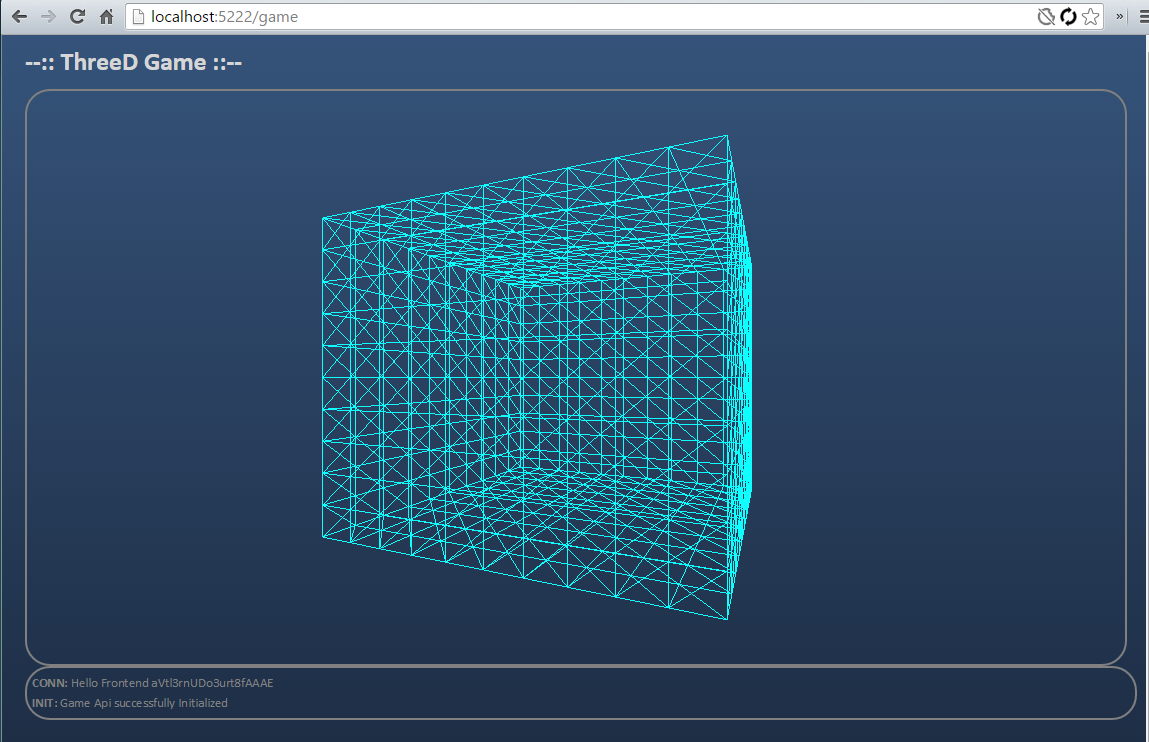
\includegraphics[width=12cm]{./images/FrontendInit.png}}
		\caption{Nicht ausgelastet Bar}
		\label{fig:FrontendInit}
\end{figure}

Lorem ipsum dolor sit amet, consetetur sadipscing elitr, sed diam nonumy eirmod tempor invidunt ut labore et dolore magna aliquyam erat, sed diam voluptua. At vero eos et accusam et justo duo dolores et ea rebum. Stet clita kasd gubergren, no sea takimata sanctus est Lorem ipsum dolor sit amet. Lorem ipsum dolor sit amet, consetetur sadipscing elitr, sed diam nonumy eirmod tempor invidunt ut labore et dolore magna aliquyam erat, sed diam voluptua. At vero eos et accusam et justo duo dolores et ea rebum. Stet clita kasd gubergren, no sea takimata sanctus est Lorem ipsum dolor sit amet.(siehe Abbildung \ref{fig:FrontendInit}).
\\
Lorem ipsum dolor sit amet, consetetur sadipscing elitr, sed diam nonumy eirmod tempor invidunt ut labore et dolore magna aliquyam erat, sed diam voluptua. At vero eos et accusam et justo duo dolores et ea rebum. Stet clita kasd gubergren, no sea takimata sanctus est Lorem ipsum dolor sit amet. Lorem ipsum dolor sit amet, consetetur sadipscing elitr, sed diam.

\section{Methodik}
\subsection{Projektmanagement}
Das Team besteht aus 5 Projektmitgliedern. Die Verteilung der Aufgaben ist in Tabelle \ref{table:Aufgabenverteilung} aufgestellt.
Verschiedene Aufgaben sind im Gitlab erfasst und Personen zugewiesen. Ein wöchentliches persönliches Treffen aller Projektmitglieder führt zu einer guten Arbeitsmoral und hohen Effektivität.
\subsubsection{GitLab}
Das Projekt wurde auf einem eigenen GitLab gehostet und den Projektmitgliedern zur Verfügung gestellt. Die Issues des Systems wurden genutzt um Aufgaben zu verteilen und zu dokumentieren.
\\
Strukuriert wurde das Arbeiten nach Feature Branches, um das Arbeiten am Projekt möglichst flexibel zu halten. Der Master-Branch diente als Release-Branch, in den regelmäßig die Änderungen per Merge Request eingetragen und getestet wurden.
\definecolor{blau}{HTML}{217AA2}
\begin{table}
	\label{table:Aufgabenverteilung}
	\centering
		\caption{Matrix der Aufgabenverteilung}
		\begin{tabular}{| L{2.6cm} | C{2cm} | C{2cm} | C{2cm} | C{2cm} | C{2cm} |}
		\hline
		\rowcolor{blau}
		\textcolor{white}{\textbf{Aufgabe}} & \textcolor{white}{\textbf{Schleiss}} & \textcolor{white}{\textbf{Grothknopf}} & \textcolor{white}{\textbf{Schiwkowksi}} & \textcolor{white}{\textbf{Hofmann}} & \textcolor{white}{\textbf{Heinrichs}}\\\hline
		Recherche 		& X & X	& X	& X	& X	\\\hline
		Konzept 		& X & X	& X	& X	& X	\\\hline
		Serverdesign	& 	& X & 	& 	& X \\\hline
		Networking		& 	& X	& 	& X	& X	\\\hline
		GameAPI 		& 	& X	&	&	& X	\\\hline
		DemoGame 		& X	&	&	&	& X	\\\hline
		ClientFrontend 	& X	&	& X	&	&	\\\hline
		ClientBackend 	& X	&	& X	&	&	\\\hline
		Database 	    & 	&	&	& X	& 	\\\hline
		Poster          & 	& 	& 	& 	& 	\\\hline
		Documentation   & 	& 	& 	& 	& X \\\hline
		Projektmgmt. 	&	&	&	& 	& X	\\\hline
	\end{tabular}
\end{table}

\subsection{Technologien} %% TODO: Dennis
\begin{figure}[H]
\begin{minipage}[t]{0.4\textwidth}
\vspace{0pt}
\paragraph{NodeJS / Javascript}\mbox{}\\
NodeJS ist eine Laufzeitumgebung für JavaScript und basiert auf der Chrome's V8 JavaScript engine. 

\end{minipage}
\hfill
\begin{minipage}[t]{0.5\textwidth}
\vspace{0pt}
\paragraph{HTML 5}\mbox{}\\
In diesem Projekt setzen wir auf HTML5 um die Sensordaten der Geräte auszulesen. Dies ist durch das neue HTML5 einfach umzusetzen.
\end{minipage}
\end{figure}

\subsubsection{Javascript Bibliotheken}

\begin{figure}[H]
\begin{minipage}[t]{0.4\textwidth}
\vspace{0pt}
\paragraph{jQuery}\mbox{}\\
jQuery ist ein schnelles, kleines und feature-rich-JavaScript-Bibliothek. Es macht die Dinge wie HTML-Dokument-Traversal und Manipulation, Ereignisverarbeitung, Animation und Ajax mit einer einfach zu bedienendes API, die über eine Vielzahl von Browsern funktioniert viel einfacher. Mit einer Kombination aus Vielseitigkeit und Erweiterbarkeit, hat jQuery die Art und Weise, dass Millionen von Menschen zu schreiben JavaScript geändert.
\end{minipage}
\hfill
\begin{minipage}[t]{0.5\textwidth}
\vspace{0pt}
\paragraph{require.js}\mbox{}\\
RequireJS ist eine JavaScript-Datei und Modul-Lader. Es ist für die In-Browser-Einsatz optimiert, aber es kann in anderen JavaScript-Umgebungen wie Rhino und Knoten verwendet werden. Mit Hilfe eines modularen Script loader wie RequireJS wird die Geschwindigkeit und Qualität des Codes zu verbessern.
\end{minipage}
\end{figure}


\begin{figure}[H]
\begin{minipage}[t]{0.4\textwidth}
\vspace{0pt}
\paragraph{socket.io}\mbox{}\\
Socket.IO ist eine JavaScript-Bibliothek für Echtzeit-Web-Anwendungen. Es ermöglicht Echtzeit, bidirektionale Kommunikation zwischen Web-Clients und Servern. Es besteht aus zwei Teilen: einem Client-seitige Bibliothek, die im Browser läuft und eine serverseitige Bibliothek für node.js. Beide Komponenten haben eine nahezu identische API. Wie node.js Es ist ereignisgesteuert.
////
Socket.IO nutzt in erster Linie die WebSocket-Protokoll mit Polling als Fallback-Option, [2] und gleichzeitig die gleiche Schnittstelle. Obwohl es einfach als Wrapper für WebSocket verwendet werden, bietet es viele weitere Funktionen, einschließlich der Rundfunk mehrere Steckdosen, die Speicherung von Daten mit jedem Kunden zugeordnet und asynchrone I / O.

Es kann mit dem NPM-Tool installiert werden. [3] [4]
\end{minipage}
\hfill
\begin{minipage}[t]{0.5\textwidth}
\vspace{0pt}
\paragraph{MongoDB}\mbox{}\\
MongoDB (abgeleitet vom engl. humongous, „gigantisch“) ist eine Schema-freie, dokumentenorientierte Open-Source-Datenbank, die in der Programmiersprache C++ geschrieben ist.[1][2] Da die Datenbank dokumentenorientiert ist, kann sie Sammlungen von JSON-ähnlichen Dokumenten verwalten. So können viele Anwendungen Daten auf natürlichere Weise modellieren, da die Daten zwar in komplexen Hierarchien verschachtelt werden können, dabei aber immer abfragbar und indizierbar bleiben.
////
Die Entwicklung von MongoDB begann im Oktober 2007 durch das Unternehmen 10gen, welches am 27. August 2013 in MongoDB, Inc. umbenannt wurde. [3] Die Erstveröffentlichung fand im Februar 2009 statt.[4] MongoDB war 2012 die am weitesten verbreitete NoSQL-Datenbank.[5]
\end{minipage}
\end{figure}



\subsubsection{Hardware}
Smartphone Controller, Platformunabhängig Node Server

%
% -----------------Implementierung-------------------------
%

\section{Implementierung}


\subsection{Architektur}

\begin{figure}[h]
	\centering
		\fbox{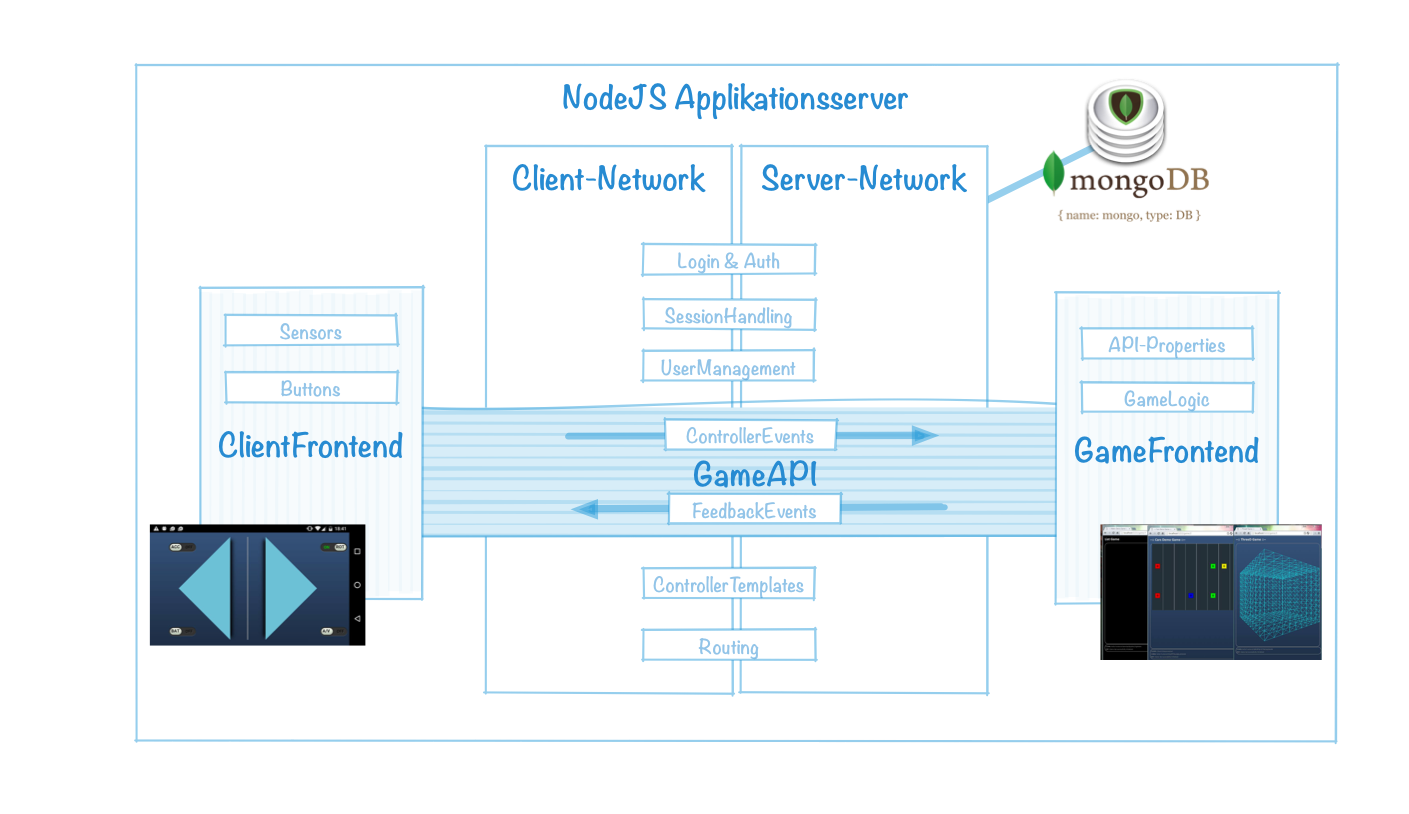
\includegraphics[width=15cm]{./images/arch/M113.png}}
		\caption{Virtuelle Maschinen vs. Docker Container\cite{dockercontainer}}
		\label{fig:dockerVM}
\end{figure}

\subsection{Network}
Die Netzwerkverbindungen bilden einen wichtigen Bestandteil der Anwendung. Alle Clients und das Server-Frontend bzw. Spiel verbinden sich zum Server via WebSocket.

\subsubsection{socket.io}
Zum Aufbau und Handling der Netzwerkverbindungen wird die Bibliothek socket.io von Guillermo Rauch verwendet. Sie kapselt die WebSocket API Spezifikationen und bietet eine vereinfachte und einfach zu benutzende API zu den WebSockets auf Client und Server-Seite. Außerdem verfügt sie über Failover-Strategien, die das Verwenden von anderen Protokollen vorsehen, für den Fall, dass WebSockets vom Client oder Server nicht unterstützt werden.
Auf node Server Seite werden die Pakete 'http' und 'socket.io' benötigt. Erstes um einen HTTP-Server zu erstellen und letzteres, um diesen dann zu einer WebSocket Verbindung aufzuwerten und diese dann zu verwalten. Grundlegen wird die Verbindung mit Hilfe von message Events implementiert, welche auf dem jeweiligen Socket ausgelöst und abgehört werden können. Dieses Prinzip ähnelt stark den von node bekannten Events. Eine Client-Version von socket.io wird vom Server automatisch veröffentlich und kann so auf dem Client direkt eingebunden und verwendet werden.
\url{https://davidwalsh.name/websocket}

\subsubsection{Server Network handling}
Die Anwendung besteht aus einem zentralen node Server, einem Frontend zur Darstellung des Spiels und eine unbestimmte Anzahl an mobilen Clients. Alle Komponenten stellen jeweils eine Websocket Verbindung zum Server her, dem so jeden Client bekannt ist und er diese verwalten kann. Durch die Verwendung der selbst geschriebenen Module 'gameApi' und 'clientNetwork' werden die Funktionen der Websockets erneut gekapselt und ermöglichen eine sehr einfaches Aufbauen der Verbindung und Verwendung der anwendungs-spezifischen Befehle.\\
Der Server hält zu jeder Zeit eine Liste aller offenen Socket-Verbindungen, die es ermöglich individuell mit jedem Client und dem Frontend zu kommunizieren. Eingehende Nachrichten können so direkt einem Absender zugeordnet werden, ohne dass dieser seine Identität oder IP-Adresse mitsenden muss.\\
Auf diesem Level der Kommunikation wurden grundlegende Socket-Events zum Verbindungsaufbau, der Nutzerverwaltung (Registration und Login) sowie dem Verschicken der eigentlichen Nachrichten. Abhängig vom Typ der eingehenden Nachricht werden die Funktionen der nächst-höheren Programmschicht aufgerufen, die diese dem Netzwerk Modul bei der Initialisierung per Callback übergeben hat. Die eigentlichen Socket-Events werden an dieser Stelle nicht weitergegeben, um die technische Socket-Logik komplett im Modul zu kapseln. Die Struktur der einzelnen Nachrichtentypen wurde genau definiert. Besonders im Fall der tatsächlichen Nachtrichten Pakete wurde ein weiteres 'type' Attribut eingefügt, die es dem Spieleentwickler erlaubt unabhängig von den Socket Event Typen eigene Nachrichten-Typen zu definieren, die zwischen Kontroller und Spiel ausgetauscht werden.\\
Ein weiterer wichtiger Aspekt ist die Art und Weise in der die Socket auf Client-Seite aufgebaut werden. Da JavaScript keine echte Persistenz von Variable und Objekten über den Scope einer HTML-Seite erlaubt, wird jede bestehende Socket-Verbindung abgebrochen sobald die Seite neu oder eine andere geladen wird. Da die Kontroller-Clients ihre Funktionalität jedoch auf eine Oberfläche begrenzen stellt dies kein gravierendes Problem dar.\\
Zusätzlich bietet das 'serverNetwork' Modul eine Reihe an Funktionen an, mit den Clients und dem Frontend zu kommunizieren und diese zu verwalten. Die meisten dieser Funktion setzen das Adressieren des gewünschten Clients über dessen Socket ID voraus.\\
\url{http://stackoverflow.com/questions/7709289/how-to-pass-javascript-object-from-one-page-to-other}
\url{http://tavendo.com/blog/post/websocket-persistent-connections/}

\subsection{Session}
Die nächste Schicht nach dem Netzwerk stellt auf Server-Seite das Modul 'sessionHandling' dar. Hier werden die noch anonymen Socket-Verbindungen bzw. deren IDs mit tatsächlichen Nutzernamen und der zugrundeliegenden Nutzerverwaltung verknüpft. Dies bedeutet zunächst, dass jeder Client sich zum Benutzen der Anwendung am Server authentifizieren muss. Jede eingehende Login-Anfrage wird da das Modul 'UserManagement' weitergeleitet um die übergebenden Nutzerdaten zu verifizieren. Nach einem erfolgreichen Login werden die Daten des Nutzers in eine Liste aktiver Nutzer gespeichert und sein Nutzername wird an die nächste Schicht weiter gegeben. Alle weiteren Anfragen werden solange abgewiesen, bis sich ein Nutzer authentifiziert hat. Beim Disconnet eines Nutzers wird sein Eintrag aus der Liste gelöscht und es wird ebenfalls eine Nachricht an die nächste Programm-Schicht übergeben. Alle Nachrichten, die tatsächliche Kommunikationsdaten zwischen Clients und dem Spiel beinhalten werden direkt weitergegeben.\\
Ein Login bedeutet notwendigerweise eine zuvor erfolgte Registrierung, welche ebenfalls vom 'UserManagement' Modul verwaltet wird. Um die Registrierung jedoch nicht zu einer unnötigen Barriere in der Verwendung der Applikation zu machen, ist es ebenfalls möglich sich anonym einzuloggen. In diesem Fall wird der jeweiligen Socket-Verbindung ein zufälliger Nutzername zugewiesen. Der Vorteil eines Nutzerkontos bietet die Möglichkeit für das Spiel, weitere Daten für einen Nutzer Session übergreifend zu speichern.\\
Wie zuvor bereits angesprochen wurde, können die Socket-Verbindungen nicht über mehrere Seitenaufrufe auf dem Client bestehen bleiben. Dies bedeutet für die Login-Session, dass diese direkt an die bestehende Socket-Verbindung gekoppelt ist und beendet wird, sobald der Socket geschlossen wird.\\

\subsection{User Management}
Das \enquote{UserManagement} kümmert sich um die Verwaltung der Nutzer. Dafür stellt es Funktionen für die Registrierung, Authentifizierung sowie für das setzen und holen von Benutzerdaten zur Verfügung. Die Funktionen im \enquote{UserManagement} bekommen eine callback Funktion übergeben, welche bei einer erfolgreichen Ausführung ausgeführt wird.

\subsection{Datenbank}
Das "Database" Modul kümmert sich um die Persistente Speicherung aller anfallenden Daten. Dafür wird eine MongoDB verwendete und die für das hinzufügen, löschen, updaten und für Abfragen benötigten Funktionen zur Verfügung gestellt.

\subsection{Mobile - Sensoren und Daten}
Die Basis aller weiteren Schritte ist das Auslesen der Sensordaten eines geeigneten Gerätes, während der gesamten Entwicklung wurden hierfür Smartphones unterschiedlicher Hersteller und Generationen verwenden. Die Daten wurden auf dem Gerät gemessen, aufbereitet und als gekapselte Datenpakete an den vorgesehenen Empfänger gesandt. Die Datenaufbereitung ist ein wichtiger Schritt, um die Netzwerklast am Knotenpunkt, dem Server, möglichst gering zu halten, da mehrere Geräte gleichzeitig eine Verbindung herstellen und aufrecht erhalten können und dies zu einer Überlast des Empfängers bei unkontrolliertem Sendevolumen führt.\\
Die von der Applikation genutzten Daten sind im folgenden erläutert.
\paragraph{Touchbildschirm}
Die übliche Art der Interaktion mit einem aktuellen Smartphone, die Toucheingabe, darf natürlich nicht außer Acht gelassen werden. Da diese in der Entwicklung äußerst einfach zu implementieren ist, unteranderem über JQuerys .tap(), kann diese Eingabe als trivial angesehen und hier nicht weiter darauf eingegangen werden.
\paragraph{Rotations- und Beschleunigungssensor}
Diese Werte bilden den Kern der Applikation und sollen hier näher dargestellt werden:\\
Die Interaktion über die Bewegung des Smartphones im dreidimensionalen Raum ist intuitiv und gut für jede denkbare Aufgabe geeignet. Die Datenerhebung erfolgt dabei für gewöhnlich durch Differentialkondensatoren und Drei-Achsen-Gyroskope.
Da die Daten vom Gerät kontinuierlich in festgelegten Intervallen bestimmt werden, können diese auf komfortable Art und Weise ausgelesen werden. Die aufwändigere Arbeit ist die anschließende Verarbeitung und Filterung der Daten. Dies geschieht über ein zu setzendes Event, namentlich das \enquote{devicemotion} -Event, das bei jeder Änderung der Rotation oder Beschleunigung feuert und seine Daten beispielhaft in der Form event.acceleration.x; oder event.accelerationRate.alpha; bereitstellt, ebenso wie das Intervall der gemessenen Daten (in Millisekunden) über event.interval; verwendet werden kann.
%\begin{figure}[h]
%  \centering
%    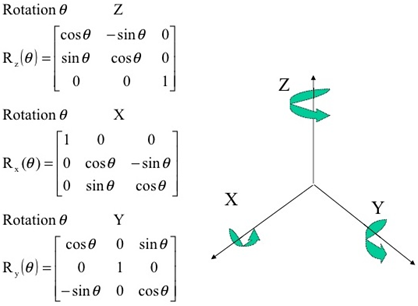
\includegraphics{images/rotation}
%     \caption{Rotationsachen dargestellt}
%\end{figure}

Die Originalversion der Rotation und Berechnungen sind zu finden in den Aufzeichnungen von Damian Gordon\footnote{\url{http://de.slideshare.net/DamianGordon1/3d-robot-movements}}.
Die Aufbereitung der Daten geschieht über eine Filterung aller leeren und ungültigen Daten, außerdem aller Daten, die darauf schließen lassen, dass keine Bewegung stattfand. Um eine Überlast der Datenverbindung zu verhindern wird eine Mittelung der ausgelesenen Daten als adäquates Mittel angesehen, diese kann über eine festgelegte Anzahl der Werte vorgenommen werden. Da Smartphones allerdings in einem unterschiedlichen Intervall Daten Messen, in der Entwicklung wurde eine Messung im Abstand von 50ms, 100ms und 200ms festgestellt, kann die Mittelung auch über einen gewissen Zeitwert vorgenommen werden.

\paragraph{Ausrichtung des Gerätes}
Die Orientierung des Gerätes wird als „Portrait“ oder „Landscape“, also vertikale oder horizontale Ausrichtung beschrieben. Diese Daten verwenden dieselbe Technik wie der Beschleunigungssensor und wird beispielsweise in der Bildschirmausrichtung verwendet. So einfach wie das Prinzip ist auch die Verwendung: Die Ausrichtung lässt sich über window.orientation; (in Grad) ausmessen. Ein Wert über 180 beschreibt dabei den Portraitmodus, über 180 den Landscape- oder Landschaftsmodus.


\begin{figure}[H]
\begin{minipage}[t]{0.4\textwidth}
\vspace{0pt}
\paragraph{Bild und Tonaufzeichungen}\mbox{}\\
Da dies einer der komplexeren Datentypen ist, den man mit dem Handy aufzeichnen kann, empfiehlt sich für die Aufnahme eine leicht benutzbare API. Mit getUserMedia() ist für Bild und Ton nun eine einfache Alternative verfügbar, die Stückweise in die aktuelle Browsergeneration eingefügt wird. Die aktuelle Verfügbarkeit innerhalb der Browser kann auf caniuse.com eingesehen werden und ergibt folgendes Bild:

\end{minipage}
\hfill
\begin{minipage}[t]{0.5\textwidth}
\vspace{0pt}
    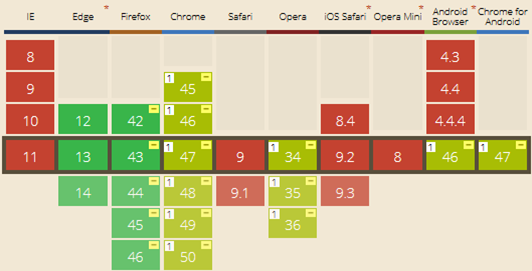
\includegraphics[width=8.5cm]{images/caniuseGetUserMedia}
     \caption{Unterstützung der getUserMedia API auf caniuse.com}
		\label{fig:test2}
\end{minipage}
\end{figure}

%\begin{figure}[h]
%  \centering
%    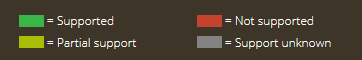
\includegraphics{images/legende}
%     \caption{Legende:}
%\end{figure}


\begin{figure}[H]
\begin{minipage}[t]{0.4\textwidth}
\vspace{0pt}
\paragraph{Batteriestatus}\mbox{}\\
Eine weitere Datenquelle ist der aktuelle Ladestatus (aktiv/inaktiv), die Batterieladung in Prozent und die Zeit zu vollständigen Ladung oder Entladung. Dies wird realisiert über die Battery Status API, die aktuell eine ähnliche Browserabdeckung erreicht wie die getUserMedia()-API.\\
Die Verarbeitung der Daten geschieht hier wie in der Rotations- und Beschleunigungsmessung über EventListener, die jeweils auf die Events chargingchange, levelchange, chargingtimechange und dischargingtimechange reagieren und nach dem Schema battery.level; die gesuchten Daten ausgeben.

\end{minipage}
\hfill
\begin{minipage}[t]{0.5\textwidth}
\vspace{0pt}
    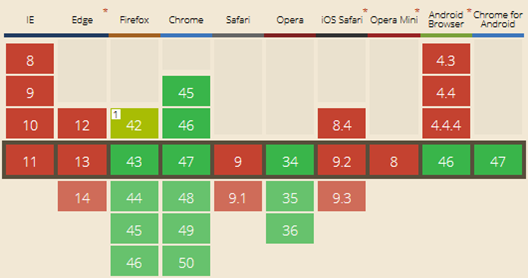
\includegraphics[width=8.5cm]{images/caniuseBatteryStatusAPI}
     \caption{Unterstützung der Battery Status API auf caniuse.com}
		\label{fig:test2}
\end{minipage}
\end{figure}

\paragraph{Vibration}
Im Gegensatz zu den anderen Daten geht es hierbei nicht um eine Ein-, sondern um eine Ausgabemethode. Die Benachrichtigung über Vibrationen ist in JavaScript denkbar einfach gestaltet, ist aber, ebenso wie die vorherigen APIs, nicht in jedem Browser verfügbar. Der letztliche Aufruf der Funktion geschieht über den Navigator, explizit über window.navigator.vibrate(), wobei die Länge und Art der Vibration angegeben werden kann.

\paragraph{Browserempfehlung}
Da (noch) nicht alle Browser alle APIs unterstützen, soll hier eine Empfehlung zur Verwendung der oben genannten Funktionalitäten genannt werden. Sowohl auf dem Desktop-Rechner als auch unter Android ist derzeit die aktuelle Version von Firefox (43) am 15.12.2015 erschienen und in der Lage, alle genannten Funktionen und APIs auszuführen.

\subsection{Template} %% TODO: Ron
\subsection{Client-JS} %% TODO: Ron

\subsection{Beschreibung der GameAPI} %% TODO Micha
Lorem ipsum dolor sit amet, consetetur sadipscing elitr, sed diam nonumy eirmod tempor invidunt ut labore et dolore magna aliquyam erat, sed diam voluptua. At vero eos et accusam et justo duo dolores et ea rebum. Stet clita kasd gubergren, no sea takimata sanctus est Lorem ipsum dolor sit amet. Lorem ipsum dolor sit amet, consetetur sadipscing elitr, sed diam.


\section{Demonstration}
\subsection{Vorbereitung}
\begin{enumerate}
 \item Ein Computer stellt den NodeJS Server.
 \item Ein weiterer Computer stellt das gewählte Demogame-Frontend auf einem großen Bildschirm dar.
 \item Mehrere Clients verbinden sich mit ihren mobilen Geräten auf den Server.
\end{enumerate}
Anschließend müssen die vom NodeJS Server benötigten Abhgängikeiten installiert werden. Dies geschieht mit einen Skriptaufruf, wie in Listing \ref{lst:installDeps} beschrieben.
\lstset{
  numbers=left,
  stepnumber=5,
  firstnumber=1,
  numberfirstline=true
}

\subsection{Start der Applikation}
Der NodeJS Server wird mit dem Befehl wie in Listing \ref{lst:launchSuccess} gestartet. Imfolgenden sollte eine Meldung erscheinen welche den Applikationsserver als gestartet meldet. Eine Beispielhafte Meldung in in Listing \ref{lst:launchSuccess} zu sehen.

\begin{figure}[h!]
	\centering
        \begin{lstlisting}[language=JavaScript,caption={Start der Applikation},label={lst:launchSuccess}]
            node NodeServer/bin/www
            16 Jan 14:39:22 serverNetwork | Server listening on port 5222
        \end{lstlisting}
\end{figure}
\subsection{Nutzen einer Demo Applikation}

\begin{figure}[H]
\begin{minipage}[t]{0.4\textwidth}
\vspace{0pt}
\paragraph{Controller Interface}\mbox{}\\
Die Clients rufen die Adresse des Servers auf und es wird ihnen eine Login Anzeige dargestellt. Hier wird nun eine Entscheidung getroffen, ob ein Login erstellt, genutzt oder anonym weiter fortgefahren werden soll.
Wird ein Login genutzt, wird anstelle eines generierten Namens der tatsächliche Benutzername im gewählten Demogame angezeigt.

\end{minipage}
\hfill
\begin{minipage}[t]{0.5\textwidth}
\vspace{0pt}
    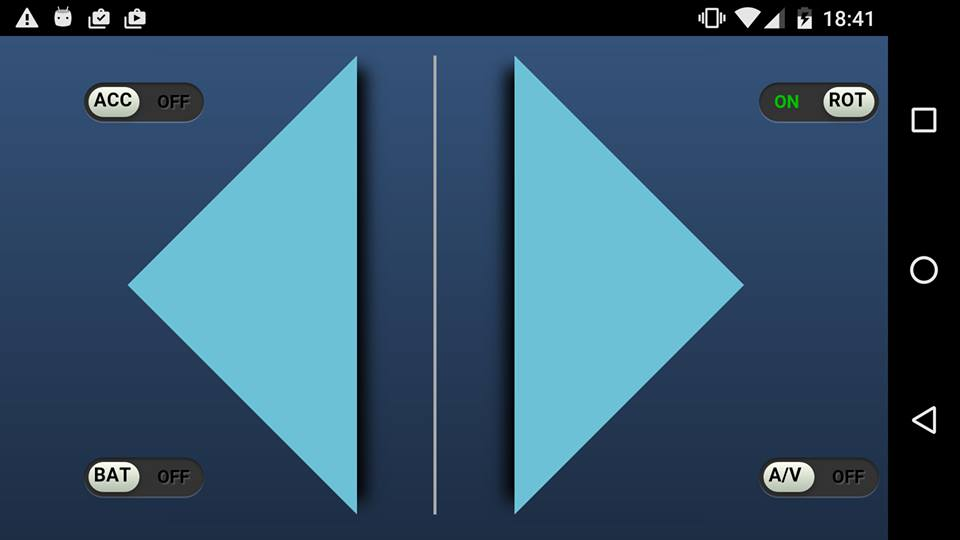
\includegraphics[width=8.5cm]{images/controllerLayoutModern}
     \caption{Unterstützung der getUserMedia API auf caniuse.com}
		\label{fig:test2}
\end{minipage}
\end{figure}



\begin{figure}[H]
\begin{minipage}[t]{0.4\textwidth}
\vspace{0pt}
\paragraph{Demo Applikation}\mbox{}\\
Die nun verbundenen Clients führen mit ihren Geräten unterschiedliche Aktionen durch. Ein Druck auf einen der Buttons auf einem der Clientgeräte wird als solcher identifiziert und im Frontend dargestellt. Ein anderer Cleint aktivert die Rotationserfassung und die gesendeten Daten erscheinen auf dem Fronend.

\end{minipage}
\hfill
\begin{minipage}[t]{0.5\textwidth}
\vspace{0pt}
    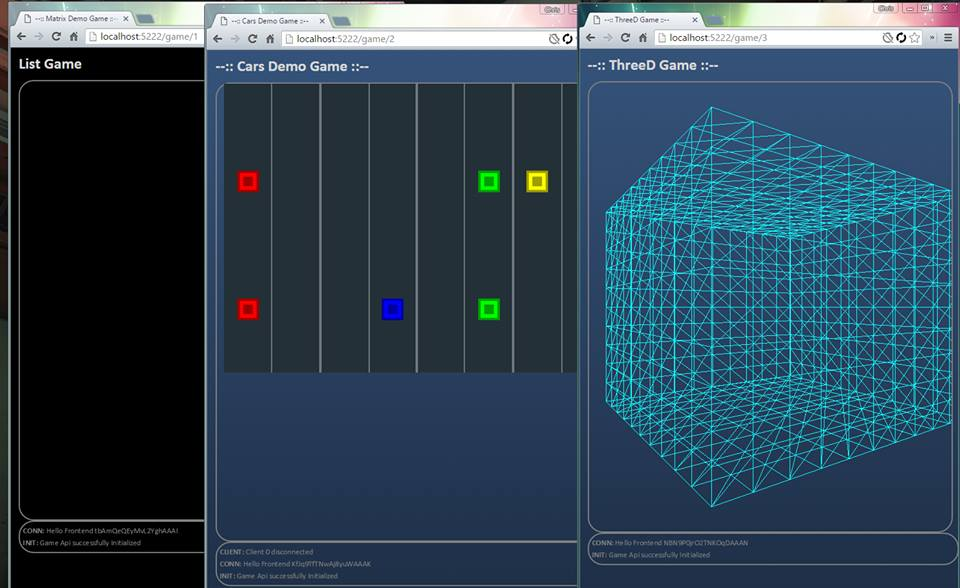
\includegraphics[width=8.5cm]{images/demoGames}
     \caption{Unterstützung der getUserMedia API auf caniuse.com}
		\label{fig:test2}
\end{minipage}
\end{figure}







\section{Lasttestmessung}\label{Lasttestmessung} %% TODO: Dennis

\subsection{Server}

\paragraph{Szenario} 
Der Server wird nach und nach mit immer mehr Paketen belastet und die CPU-Auslastung ermittelt.

\begin{figure}[H]
\begin{minipage}[t]{0.4\textwidth}
\vspace{0pt}
\paragraph{Durchführung}\mbox{}\\
Mithilfe des node-inspectors\footnote{https://github.com/node-inspector/node-inspector} wurde die NodeJS-Serveranwendung analysiert. Der node-inspector ermöglicht eine Nutzung der Entwicklertools des Chrom-Browsers. Zur Ermittlung der CPU-Last wurden Profile bei verschiedenen Lastzuständen erstellt welche 30 Sekunden lang aufrecht erhalten wurden.

\end{minipage}
\hfill
\begin{minipage}[t]{0.5\textwidth}
\vspace{0pt}
	\centering
	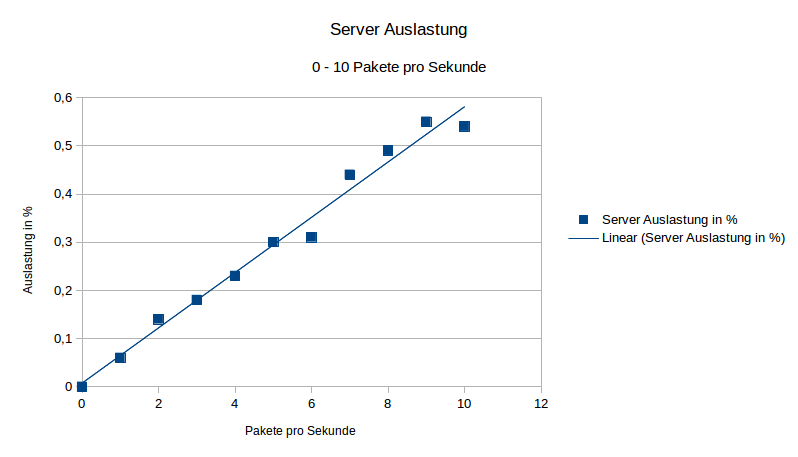
\includegraphics[width=1\textwidth]{./images/ServerLast1.png}
	\caption{ServerLast1}
	\label{fig:ServerLast1}
\end{minipage}
\end{figure}

\begin{figure}[H]
\begin{minipage}[t]{0.4\textwidth}
\vspace{0pt}
\paragraph{Ergebnisse}\mbox{}\\
Anhand der Ergebnisse ist gut der lineare Anstieg der Auslastung zu erkennen. Das Diagramm \ref{fig:ServerLast1} zeigt Messwerte bei 0 - 10 Paketen und das Diagramm \ref{fig:ServerLast2} stellt die Ergebnisse von 0 bis 5500 Paketen da. Auf dem Diagramm \ref{fig:ServerLast2} ist gut zu erkennen das die Auslastung ab ca. 3500 Paketen in einem geringerem maße ansteigt, allerdings ist auch hier ein linearer Verlauf zu erkennen. Die Auslastung schwankt zwar je nach eingesetzten System, der lineare Anstieg wird sich übertragen lassen. Um dies zu bestätigen sind weitere Messungen auf verschiedenen Testsystemen nötig.

\end{minipage}
\hfill
\begin{minipage}[t]{0.5\textwidth}
\vspace{0pt}
	\centering
	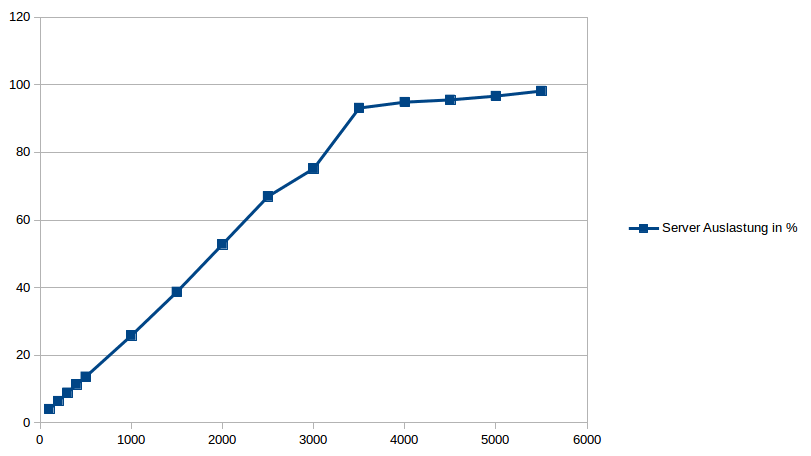
\includegraphics[width=1\textwidth]{./images/ServerLast3.png}
	\caption{ServerLast2}
	\label{fig:ServerLast2}
\end{minipage}
\end{figure}


%\begin{table}
%	\label{table:CPUMesswerte}
%	\centering	
%	\begin{tabular}{| L{2cm} | L{2cm} | L{2cm} |}
%		\hline
	%	\rowcolor{blau}
	%	\textcolor{white}{\textbf{Pakete/sec}} & \textcolor{white}{\textbf{CPU Last in \% (Server)}} & \textcolor{white}{\textbf{CPU Last in \% (Client)}} \\\hline
%		0 	& 0,00	& \\\hline
%		1 	& 0,06 	& \\\hline
%		2 	& 0,14	& \\\hline
%		3 	& 0,18	& \\\hline
	%	4 	& 0,23	& \\\hline
	%	5 	& 0,30	& \\\hline
	%	6 	& 0,31	& \\\hline
	%	7 	& 0,44	& \\\hline
	%	8 	& 0,49	& \\\hline
	%	9 	& 0,55	& \\\hline
	%	10 	& 0,54	& \\\hline
	%	100 & 3,45	& \\\hline
%	\end{tabular}
%	\caption{CPU Messwerte}
%\end{table}

\subsubsection{Frontend}

\paragraph{Test Szenario} Zur Messung der Latenz wird ein Gerät mit dem Server verbunden und jede Sekunde dessen durchschnittliche Latenz vom Senden der Daten auf dem Gerät bis zur Ausgabe dieser durch die API erfasst. Die Auslastung des Servers wird durch das Senden von zusätzlichen Paketen erreicht. Die Senderate wird nach und nach gesteigert um die Maximale Auslastung der API auf dem Testsystem zu ermitteln. Zu beachten ist das auf allen Geräten vergleichbare Zeitstempel vergeben werden um die Ergebnisse nicht zu verfälschen. Die Test werden dabei ohne die Anbindung einer Anwendung an die API durchgeführt. Zu beachten ist, das diese auch Leistung benötigt was die Ergebnisse drastisch verändern kann. Aufgrund des Fokus auf die Entwicklung einer API ohne eine gezielte Anwendung wurde diese nicht berücksichtigt.


\paragraph{Durchführung}
Zur Erfassung der Daten wurde die Anzahl der gesendeten Pakete und der durchschnittlichen Latenz pro Sekunde von einem Gerät ermittelt. Während der Messung wurde der Server mit einer Unterschiedlich starken Anzahl an zusätzliche Paketen belastet um eine Höhere Auslastung zu erreichen. Die Werte wurden dabei in einem Abstand von einer Sekunde ermittelt. Zum Erfassen er Daten wurden die Chrome-Entwicklertools verwendet. Es wurden für jede Laststufe Daten über 50 Sekunden erfasst. Der Server und das Frontend liefen bei dem Test auf dem gleichen System.



\begin{figure}[H]
\begin{minipage}[t]{0.4\textwidth}
\vspace{0pt}
\paragraph{Ergebnisse}\mbox{}\\
Die Ergebnisse der Messung sind in dem Diagramm \ref{fig:LatenzMessung} zu erkennen. Der Mittelwert gibt die Durchschnittliche Latenz über 50 Sekunden an. Durch die mittlere Abweichung ist gut zu erkennen das es zu gelegentlichen Latenz Spitzen kommt, welche im Betrieb unter Umständen zu Problemen führen können. Ab einer Paketanzahl von 5000 ist ein drastischer Anstieg der durchschnittlichen Latenz zu erkennen. Bei der Annahme das ein Gerät ~100 Pakete die Sekunde versenden kann, kann im Betrieb ohne Anwendung eine auf dem Testsystem maximal mögliche Anzahl von 50 Geräten angenommen werden. Mit blick auf die Daten von der Server-Leistungsmessung\ref{fig:ServerLast2} sollte die Anzahl von 35 Geräten nicht überschritten werden und der Bereich von 35-50 Als Pufferzone eingeplant werden.

\end{minipage}
\hfill
\begin{minipage}[t]{0.5\textwidth}
\vspace{0pt}
	\centering
	\centering
	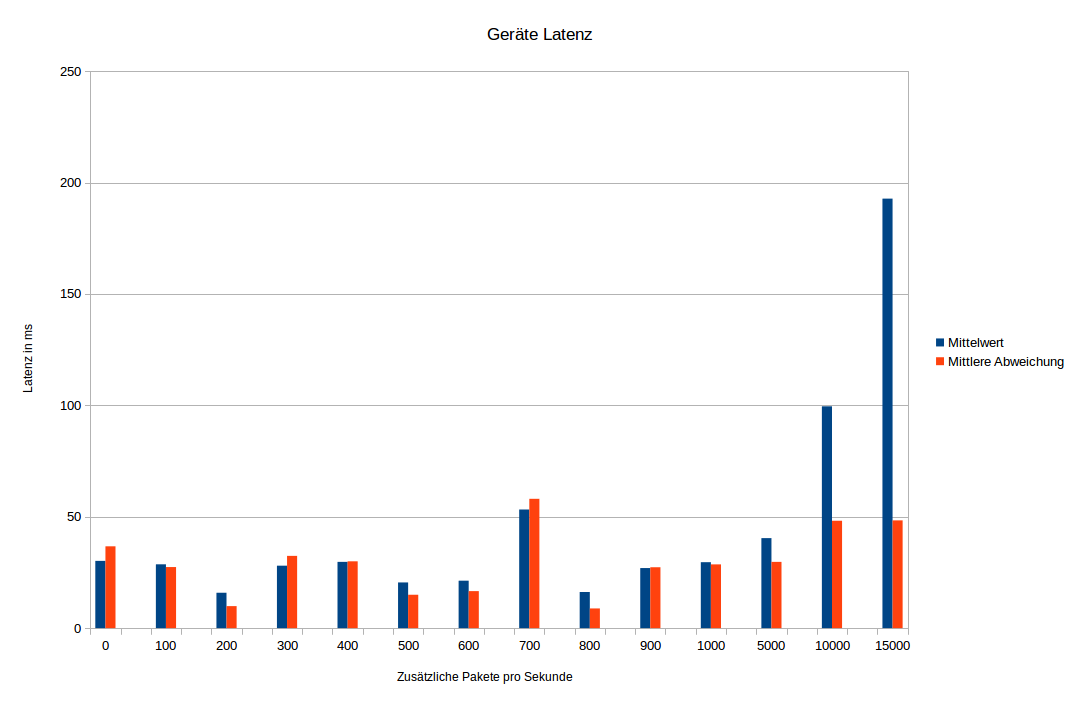
\includegraphics[width=1\textwidth]{./images/LatenzMessung.png}
	\caption{LatenzMessung}
	\label{fig:LatenzMessung}
\end{minipage}
\end{figure}


%%
%%
%%
\section{Ausblick}

\paragraph{QRCode} %% TODO: Micha
    Busstop sinnvoll, gameApi.printQRCode()
\paragraph{Glättung der Sensor Werte}  %% TODO: Dennis
Ein noch zu lösendes Problem ist die Glättung der von den Sensoren kommenden Werte. Je nach Gerät liefern die Sensoren unterschiedlich Stark schwankenden Daten. So feuert ein auf dem Tisch liegendes Gerät permanent Orientierungsdaten, obwohl es nicht bewegt wird. Diese Schwankungen müssen erkannt und unterbunden werden. Einbauen eines thresholds.

\paragraph{Begrenzung der gesendeten Sensor Daten} %%TODO: Dennis
Um den Server nicht ungleich durch die verschiedenen Geräte zu belasten und die Auslastung berechenbar zu machen, muss das Sendeverhalten reglementiert werden. Die optimalen Werte dafür müssen noch durch weitere Leistungstest ermittelt werden und hängen auch von der Anwendung ab welche an die API angebunden ist.


\section{Conclusion} %% TODO: Chris
Alles super. Die erste Million ist nah!




%%%%%%%%%%%%%%%%%%%%%%%%%%%%%%%%%%%%%%%%%%%%%%%%%%%%%%%%%%%%%
%%%%% References %%%%%
\bibliographystyle{spiebib}   %>>>> makes bibtex use spiebib.bst
\bibliography{references}   %>>>> bibliography data in report.bib

\newpage
\appendix

\end{document} 
